\section{Zadanie 1: Rozkład QR}

\subsection{Charakterystyka metody i problem}

Rozkład QR jest techniką dekompozycji macierzy \( A \) na iloczyn dwóch macierzy:
\[
A = QR,
\]
gdzie:
\begin{itemize}
    \item \( Q \) jest macierzą ortogonalną (\( Q^T Q = I \)),
    \item \( R \) jest macierzą górnotrójkątną.
\end{itemize}

Rozkład ten realizowany jest za pomocą procesu Gram-Schmidta, polegającego na ortogonalizacji kolumn macierzy \( A \). Proces ten można zapisać w postaci:
\[
q_1 = \frac{a_1}{||a_1||}, \quad 
q_k = \frac{a_k - \sum_{i=1}^{k-1} \langle a_k, q_i \rangle q_i}{||a_k - \sum_{i=1}^{k-1} \langle a_k, q_i \rangle q_i||}.
\]

Aby ocenić dokładność uzyskanego rozkładu, mierzymy błąd ortogonalności macierzy \( Q \), definiowany jako największa wartość iloczynu skalarnego dwóch różnych wektorów \( q_i \) i \( q_j \), gdzie \( i \neq j \):
\[
E = \max\{\langle q_i, q_j \rangle \; : \; i \neq j\}.
\]

Aby zmniejszyć błędy ortogonalności, można zastosować rozkład QR wielokrotnie.

\subsection{Przeprowadzane testy}

W ramach przeprowadzonych testów dokonano analizy zależności błędu ortogonalności od wielkości macierzy \( n \) dla dwóch typų macierzy, przy czym wybierano maksymalną wartość spośród iloczynów skalarnych różnych kolumn:
\begin{itemize}
    \item macierzy losowych,
    \item macierzy o dominującej przekątnej.
\end{itemize}

Dodatkowo przeanalizowano wpływ powtórnej dekompozycji QR na zmniejszenie błędów ortogonalności. Testy przeprowadzono dla macierzy o rozmiarach od \( n = 1 \) do \( n = 250 \). Dla każdej wartości \( n \) generowano 10 losowych macierzy, a wyniki uśredniano.

\begin{minipage}{0.45\textwidth}
    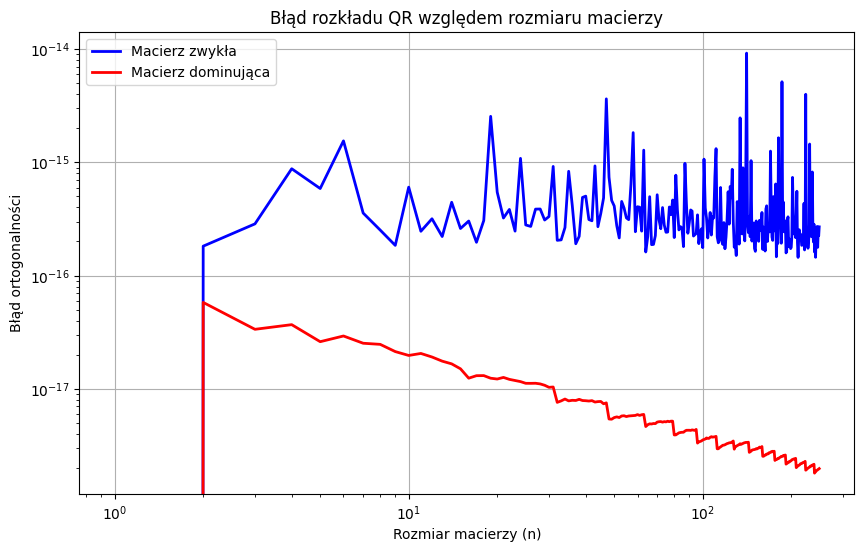
\includegraphics[width=\textwidth]{wykresy/zadanie 1/blad_rozmiar.png}
\end{minipage}
\hfill
\begin{minipage}{0.45\textwidth}
    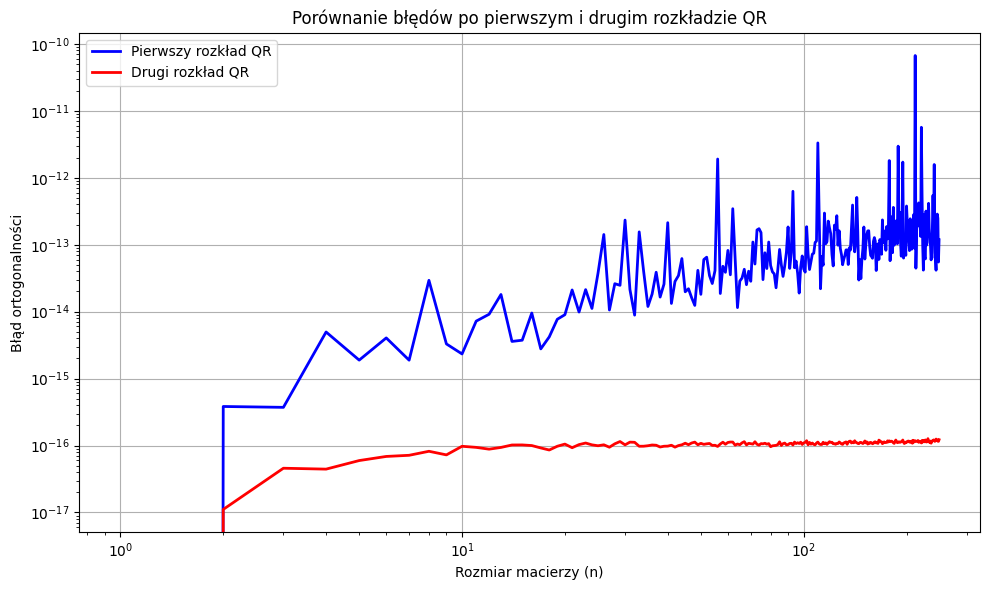
\includegraphics[width=\textwidth]{wykresy/zadanie 1/second_QR.png}
\end{minipage}

\subsection{Wyniki i analiza}
\begin{itemize}
    \item Zależność błędu ortogonalności od rozmiaru macierzy \( n \) różni się w przypadku macierzy losowych i macierzy z dominującą przekątną.
    \item Powtórna dekompozycja QR znacząco zmniejsza błędy ortogonalności, co widać na wykresie. 
\end{itemize}

\subsection{Wnioski}
\begin{itemize}
    \item Powtórna dekompozycja QR pozwala na znaczące zmniejszenie błędów ortogonalności, co może być istotne w aplikacjach wymagających wysokiej precyzji.
    \item Błędy na poziomie \( 10^{-14} \) są marginalne dla większości zastosowań, jednak w przypadku bardziej wymagających obliczeń zastosowanie dodatkowych kroków poprawy dokładności może być konieczne.
\end{itemize}
